\documentclass[journal=jacsat,manuscript=article,layout=twocolumn,12pt]{achemso}
\usepackage[version=3]{mhchem} % Formula subscripts using \ce{}
\usepackage[T1]{fontenc}       % Use modern font encodings
\usepackage{amsmath}
% NB added command for in line cite
\newcommand{\onlinecite}[1]{\hspace{-1 ex} \nocite{#1}\citenum{#1}} 
% 2 column equations
\usepackage{widetext, widetable}
%
\author{Z.~Levey}
\author{B.~A.~Laws}
\email{B.Laws@unsw.edu.au}
\author{K.~Nauta} 
\author{T.~Schmidt}

\affiliation{School of Chemistry, University of New South Wales, Sydney NSW 2052, Australia}
\title{Formation of PhenRad via CH ring insertion...}
\abbreviations{PES,PAD,EA,eKE,FWHM,VMI}
\begin{document} 
\begin{abstract} 
This is the manuscripts abstract...
\end{abstract} 
%\begin{tocentry}
%\includegraphics[width=1\textwidth]{Figures/TOC}
%\end{tocentry}

\section{Introduction}
Intro....~\cite{por20}
oconnor paper says...~\cite{oco11}



\section{Results}
Here is a figure. You can then refer to the figure using Fig.~\ref{fig1-delay}.
\begin{figure}
	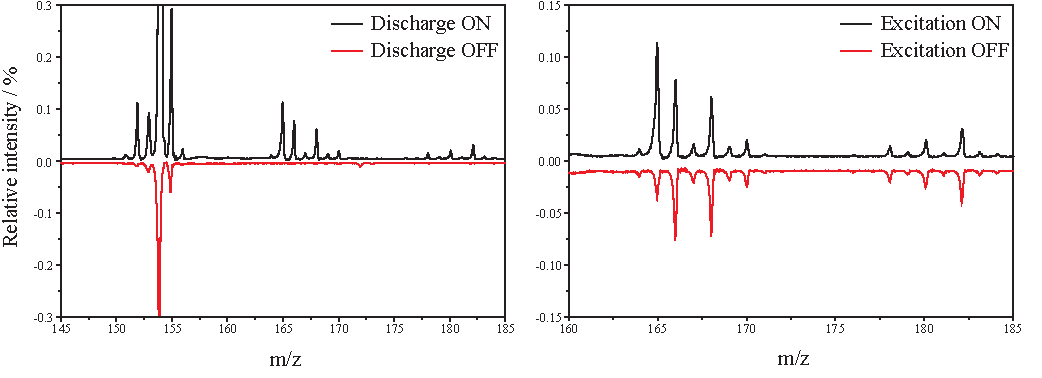
\includegraphics[width=0.5\textwidth]{Figures/discharge-exc}
	\caption{A figure showing the depletion rate for different laser delays.}
	\label{fig1-delay}
\end{figure}

\section{Discussion}
Equations may be written using general LaTeX format, and the same labelling method.
\begin{equation}
I(\theta,\epsilon) = \frac{\sigma_{\text{total}}(\epsilon)}{4\pi}[1+\beta(\epsilon)\text{P}_2(\cos\theta)],
\label{eq:beta}
\end{equation}
where $\beta$ in Eq.~(\ref{eq:beta}) is a really cool parameter.

We can also make tables, like this one, Table~\ref{tab:C2H}.
\begin{table}
	\caption{This is my table caption.} \label{tab:C2H}
	\begin{tabular}{c c c c c}
		\hline Peak & eBE (cm$^{-1}$) & $v$ (cm$^{-1}$) & $\beta$ & Symmetry \\ 
		& & & & \\\hline \hline
		& 23 591 & -231 & + & $\Sigma^+$ 
	\end{tabular}
\end{table}

\section{Conclusion}

\section{Experimental Details}


\begin{acknowledgement}
	This research was supported by the Australian Research Council Discovery
	Project Grant DP160102585. The author's thank Andrei Sanov for discussion on his modified Cooper-Zare anisotropy model.
\end{acknowledgement}


% Create the reference section using BibTeX: 
\bibliography{PhenRad}

%\newpage
%\onecolumn
%\subsection{TOC Graphic}
%\vspace{2ex}
%\begin{center}
%	\includegraphics[width=8.5cm]{Figures/TOC}
%\end{center}


\end{document}
